% !TeX root = ../main.tex

\chapter{移动操作机器人的国内外现状}
\label{cha:intro}

\section{移动操作机器人概念}
\label{cha:base_comcept}

移动操作机器人(Mobile Manipulator)目前仍然是一个非常宽泛的概念,通常我们认为,典型的移动操作
机器人是由一台机械臂和一个可自由移动的平台组成的,机械臂通过某种方式挂载在平台上\cite{bostelman2016survey}。
近年来,随着科技的飞速发展以及制造业转型的巨大压力,智能机器人方向成为新的研究热点,在学术界及
工业界受到了广泛关注\cite{schneier2015literature}。移动操作机器人已经被广泛的应用到了航天\cite{ambrose2004mobile}、医药、制造\cite{guizzo2011meka}、清洁、服务等多个场景,
在各个领域发挥着重要的作用。但移动操作机器人在性能和功能上还远远没有达到我们期待的水平,相
关研究及工业尝试还需要很长时间的发展。

广义的移动操作机器人除机械臂外,可依赖的平台非常多样,除了常见的轮式底盘、平衡车式底盘外,还可
使用无人机作为移动平台。无人机平台的移动操作机器人有夹爪式、机械臂式等各种种类,近年来也广泛的
受到各界的关注\cite{ruggiero2018aerial}。相比于无人机底盘,轮式底盘的移动操作机器人负载更
高,性能更强劲,应用更加广泛,功能更加多样,品种也更加丰富,因此本文主要论述以轮式底盘作为移动
平台的移动操作机器人,并给出相应的控制方法。

\section{移动操作机器人国内外应用现状}
\label{cha:application}

近年来,国内外机器人相关的创业公司层出不穷,智能机器人行业也是投资机构聚焦的热点。机器人
作为主要生产工具在制造业承担作用的历史非常久,机器人在制造业最早的规模化应用被认为诞生
在汽车制造领域。同其他行业相比,汽车领域产品款式固定,出货量大,规模效应强,这些特性使得基于硬编码
控制的大型高精度机械臂得到广泛应用,如图\ref{fig:armcar} 展示了工业机械臂在汽车产线上应用
的场景。以汽车工业为代表的自动化机器人应用大部分为高精度工业机械臂,其发展已经有近
半个世纪的历史,自1973年ABB和KUKA将工业机器人推向市场后,这一行业迎来了飞速发展。目前,国际
工业机器人领域有四大标杆企业,分别是瑞典 ABB、德国 KUKA、日本FANUC 和日本安川电机。四大厂商
各有所长,ABB擅长控制系统,KUKA优势在于系统集成应用与本体制造,FANUC长于数控系统,安川电机
的优势在于伺服电机制造和运动控制器的研发。除四大头部企业外,美国 Adept Technology、瑞士
Staubli、意大利Comau、日本的川崎、爱普生、那智不二越和中国新松机器人自动化股份有限公司也是
国际工业机器人的重要供应商\cite{huangxihuanReview}。除汽车工业外,高精度工业机械臂在医疗
领域也取得了不俗的成绩,Intuitive Surgical公司研发的“达芬奇”手术机器人在世界范围内广泛应用,
我国于2006年引入第一套达芬奇手术系统,至今各式手术机器人在中国已累计完成10万例外科手术,如
图\ref{fig:davinci}。

\begin{figure}
\centering
\begin{subfigure}{.5\textwidth}
  \centering
  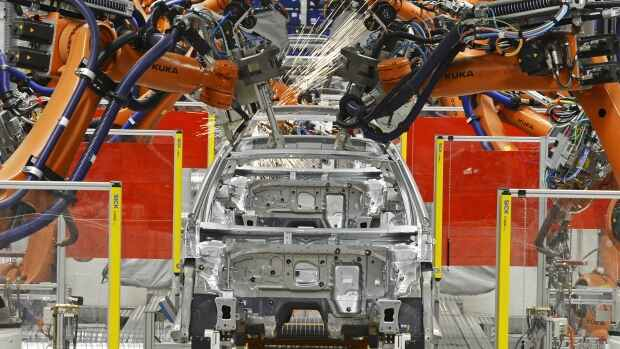
\includegraphics[height=3cm]{kuka_car.jpg}
  \caption{完全由库卡机械臂组成的汽车焊接流水线}
\end{subfigure}%
\begin{subfigure}{.5\textwidth}
  \centering
  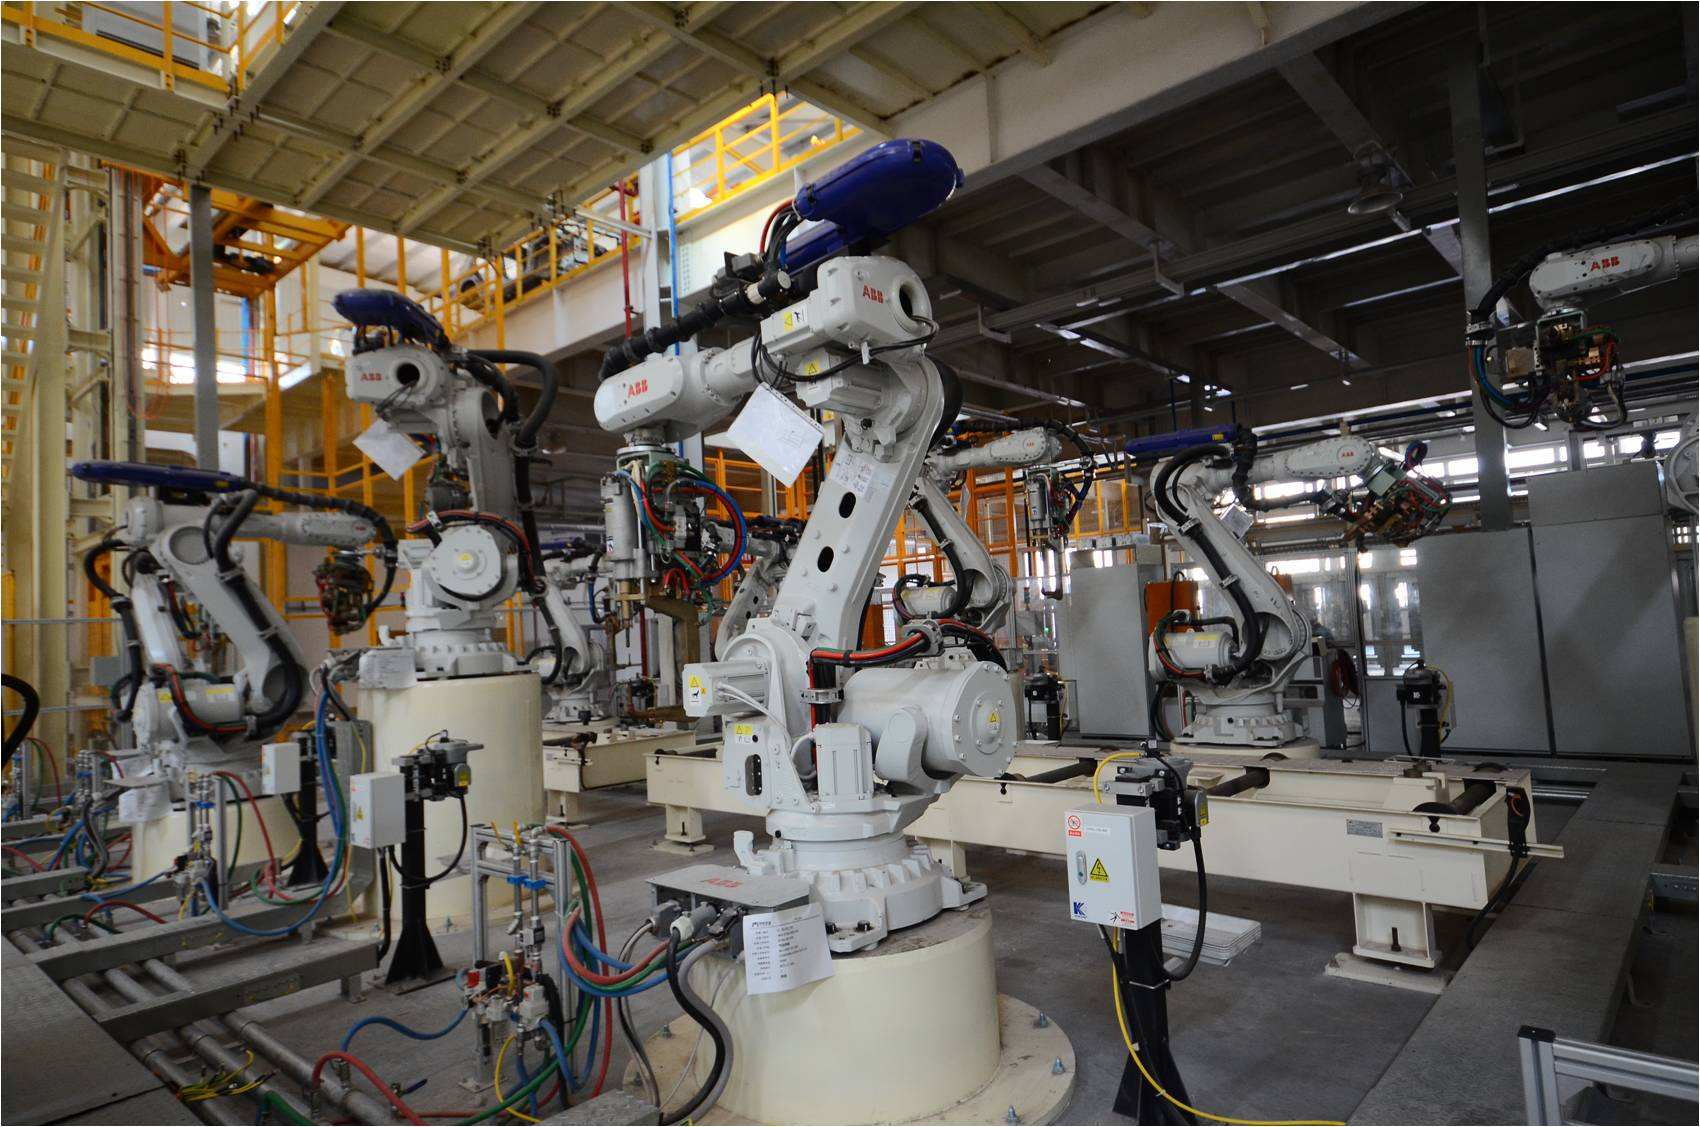
\includegraphics[height=3cm]{abb_car.jpeg}
  \caption{ABB机械臂组成的汽车零件装配产线}
\end{subfigure}
\caption{工业机械臂在流水线上工作}
\label{fig:armcar}
\end{figure}

\begin{figure}[ht] % use float package if you want it here
  \centering
  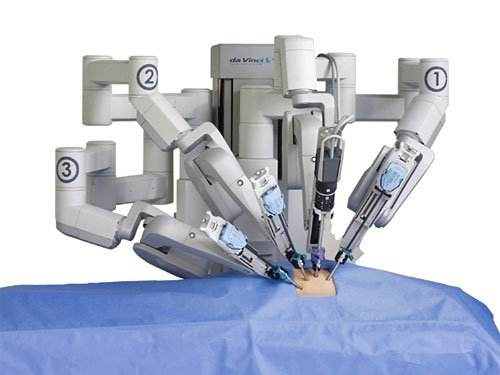
\includegraphics[width=.4\linewidth]{davinci.jpeg}
  \caption{达芬奇机器人在工作}
  \label{fig:davinci}
\end{figure}


上述这些产品注重控制精度与末端负载,功耗巨大,重量也非常可观,几乎没有移动能力。
尽管工业机器人行业至今已发展多年,体量巨大,技术积累丰厚,但企业的产品研发主要集中在
工业机械臂的硬件性能方面,如提升精度与负载,提升安全性等等。近年来随着电商、物流行业
的迅猛发展,基于机械臂的智能分捡领域开始
蓬勃发展,国内涌现出一批专注物品分捡、分类的创业公司,如深圳蓝胖子机器人\ref{fig:lanpangzi}、
北京梅卡曼德机器人\ref{fig:mechmind}等,这些企业专注于算法或者算法硬件集成,致力于
机器人的自动化与智能化。


\begin{figure}
\centering
\begin{subfigure}{.5\textwidth}
  \centering
  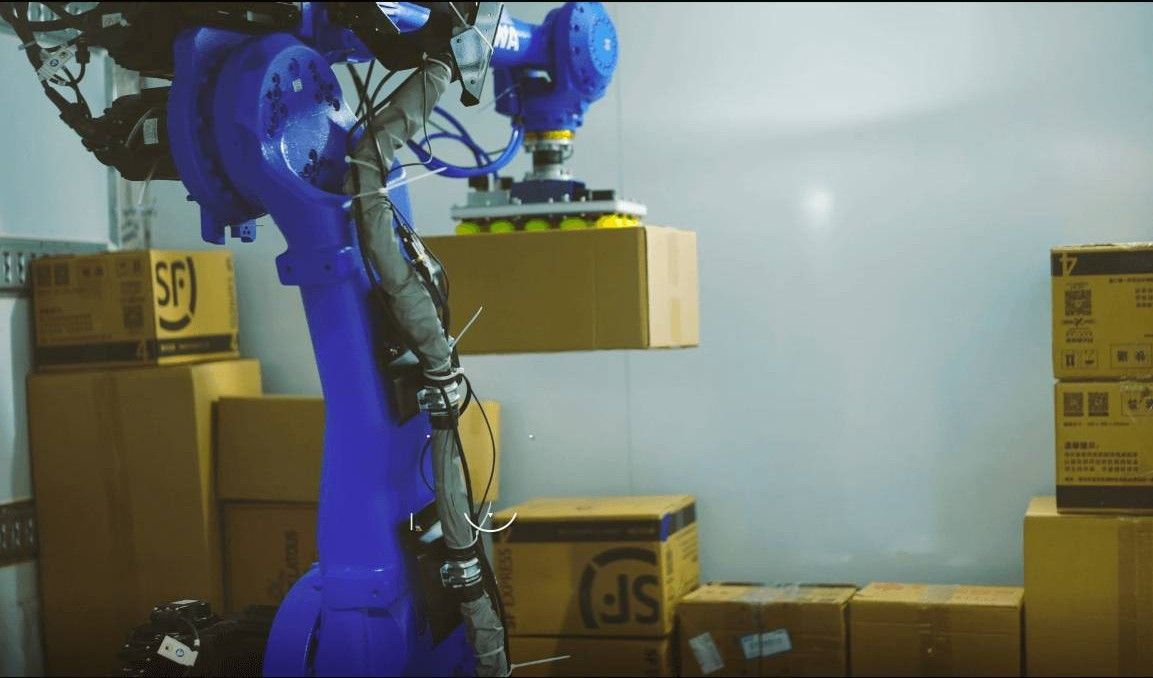
\includegraphics[height=4cm]{lanpangzi_robot.jpeg}
  \caption{蓝胖子机器人研发的机械臂分捡系统}
  \label{fig:lanpangzi}
\end{subfigure}%
\begin{subfigure}{.5\textwidth}
  \centering
  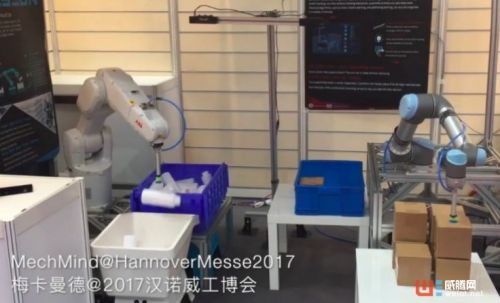
\includegraphics[height=4cm]{mechmind.jpg}
  \caption{梅卡曼德研发的机械臂操作系统在工作}
  \label{fig:mechmind}
\end{subfigure}
\end{figure}

除了专注于操作的工业机械臂,专注移动导航的自动导航车(AGV,Automated Guided Vehicles)
在制造业、运输业也大放异彩。AGV产品最早出现在上世纪50年代,于70年代左右开始应用于
制造业\cite{黄志球2010自动导航车}。按
功能可将AGV分为自动搬运车、自动拖车、自动叉车等几类,或者按照导航方式可分为电磁引导、激光引导、
惯性引导等方式。目前AGV在汽车厂(如通用、丰田、大众等)的制造和装配线上都得到了广泛的使用。
相比于工业机械臂,AGV的机械、电子结构并不复杂,控制算法也相对成熟,制造难度不大。我国的海康威视
就是一个重要的AGV生产商,如图\ref{fig:haikang}展示了海康威视研发的系列AGV产品。

\begin{figure}
\centering
\begin{subfigure}{.4\textwidth}
  \centering
  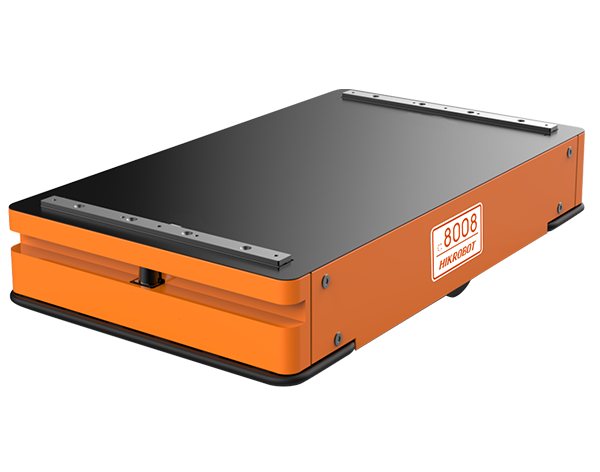
\includegraphics[width=.6\linewidth]{haikang1.png}
  \caption{移载AGV}
\end{subfigure}%
\begin{subfigure}{.4\textwidth}
  \centering
  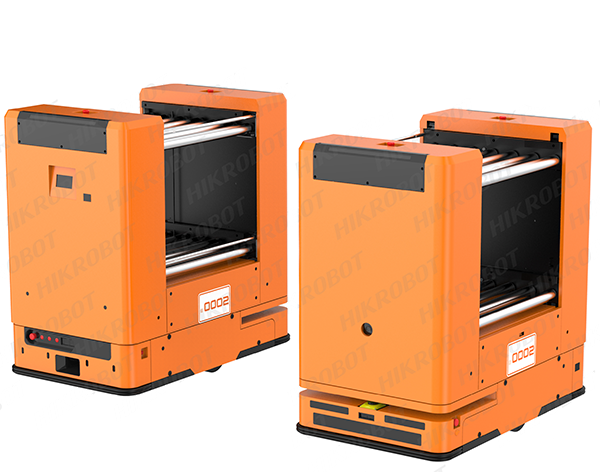
\includegraphics[width=.6\linewidth]{haikang2.png}
  \caption{移载AGV}
\end{subfigure}%
\\
\begin{subfigure}{.4\textwidth}
  \centering
  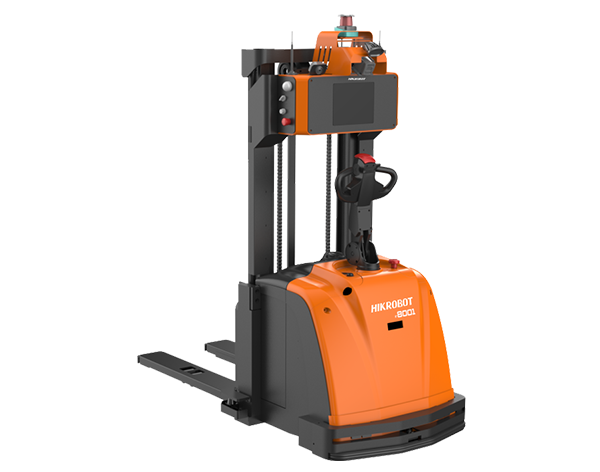
\includegraphics[width=.6\linewidth]{haikang3.png}
  \caption{叉车}
\end{subfigure}%
\begin{subfigure}{.4\textwidth}
  \centering
  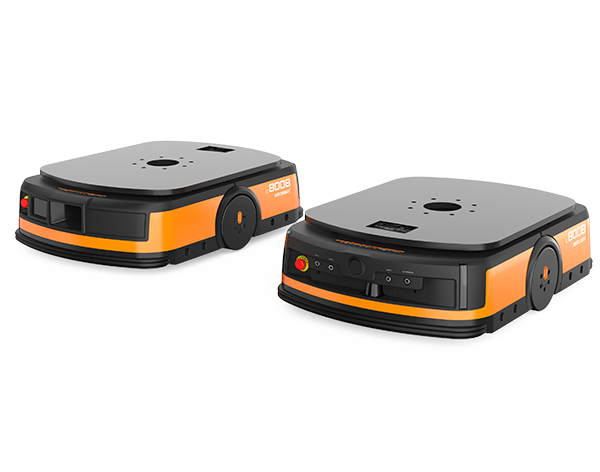
\includegraphics[width=.6\linewidth]{haikang4.png}
  \caption{潜伏系列}
\end{subfigure}%
\caption{海康威视发布的各式AGV产品}
\label{fig:haikang}
\end{figure}

移动操作机器人本质上是机械臂产品与AGV的集合,但目前来看其商业应用方向与前两者有极大的区别。
现阶段移动操作机器人领域还没有出现在商业上十分成功的厂商,但是国内外出现了一大批专注这一
领域的创业公司,致力于将移动操作机器人应用到医疗、服务、制造等场景下。例如Diligent Robotics
研发的机器人护士Moxi\ref{fig:moxi}专注于医院场景下的配送、运输业务;我国华大智造研发的远程
超声检测系统\ref{fig:huada},该系统在新冠疫情期间的武汉方舱医院内进行了应用测试\cite{wushengzheng20205g},
取得了可喜的进展。

\begin{figure}
\centering
\begin{subfigure}{.5\textwidth}
  \centering
  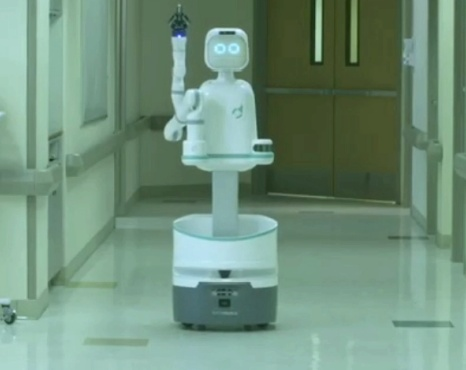
\includegraphics[height=3.5cm]{moxi.jpg}
  \caption{Moxi机器人护士}
  \label{fig:moxi}
\end{subfigure}%
\begin{subfigure}{.5\textwidth}
  \centering
  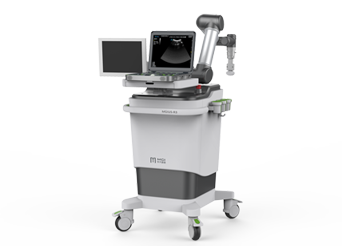
\includegraphics[height=3.5cm]{huada.png}
  \caption{华大智造的远程超声检测机器人}
  \label{fig:huada}
\end{subfigure}%
\end{figure}

除上述两例面向特定任务的移动机器人外,产业界还有一部分产品定位为“仿人”的具有社交属性的服务
机器人,例如日本Toyota公司面对人口老龄化现象推出的家庭照料机器人HSR(Human Support Robot)\ref{fig:hsr},
以及Softbank Robotic发布的Pepper机器人\ref{fig:pepper}。这些机器人大都行动笨拙,但是有双臂、
手、头等和人类身体结构对应的机械结构,并且有一定的交互能力。

\begin{figure}
\centering
\begin{subfigure}{.5\textwidth}
  \centering
  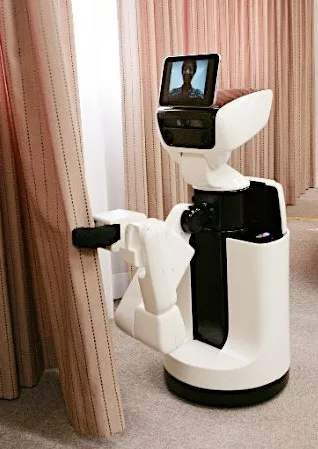
\includegraphics[height=5cm]{hsr.jpeg}
  \caption{Toyota Human Support Robot}
  \label{fig:hsr}
\end{subfigure}%
\begin{subfigure}{.5\textwidth}
  \centering
  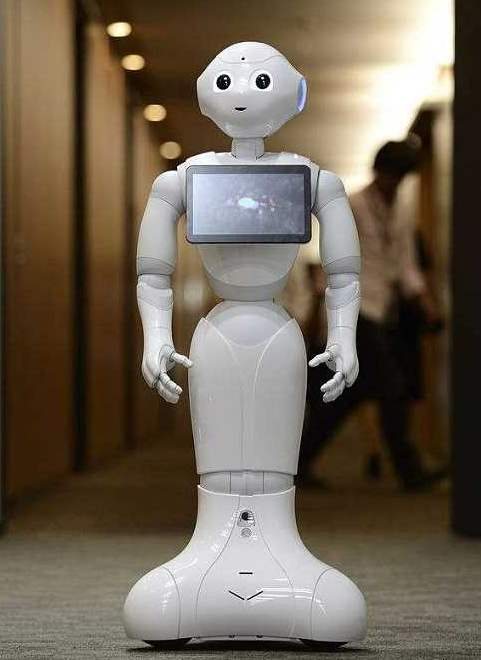
\includegraphics[height=5cm]{pepper.jpeg}
  \caption{Softbank Robotics Pepper}
  \label{fig:pepper}
\end{subfigure}
\label{fig:hsr_pepper}
\caption{仿人机器人产品}
\end{figure}

除了上述商业应用比较明确的公司以及产品外,国际上大名顶顶的波士顿动力公司(Boston Dynamics)也
研究发布了几款轮式移动操作机器人\ref{fig:bd_wheel}和以大狗为移动平台挂载轻量级机械臂的机器人\ref{fig:bd_dog}。
这些机器人在运动控制上均达到了极高的水平,为移动操作机器人的运动性能评价设定了新的标杆。

\begin{figure}
\centering
\begin{subfigure}{.5\textwidth}
  \centering
  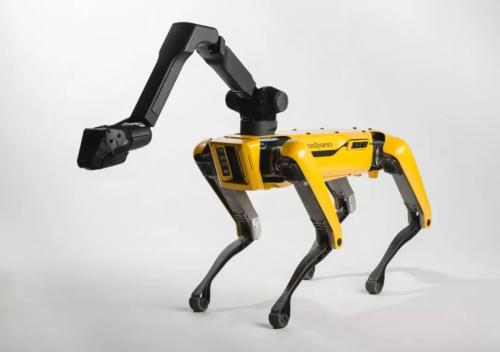
\includegraphics[width=.6\linewidth]{bd_dog.jpg}
  \caption{SPOTMINI + Arm大狗机器人}
  \label{fig:bd_dog}
\end{subfigure}%
\begin{subfigure}{.5\textwidth}
  \centering
  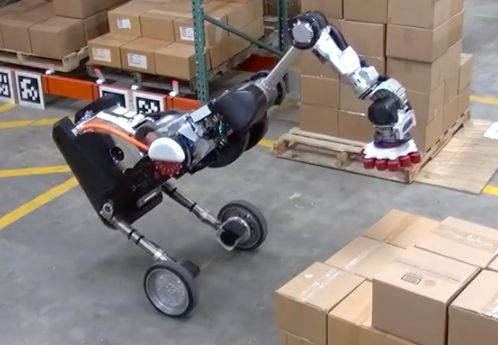
\includegraphics[width=.6\linewidth]{bd_wheel.jpg}
  \caption{仓储搬运机器人Handle}
  \label{fig:bd_wheel}
\end{subfigure}
\caption{波士顿动力发布的移动操作机器人产品}
\end{figure}


\section{移动操作机器人国内外研究现状}
\label{cha:research}

机器人领域中学术界的研究总是走在工业界前面,移动操作机器人方向也不例外。最早的工业
机械臂于1969年由Victor Scheinman发明,称为“斯坦福机械臂”,随后Victor Scheinman在
MIT AI Lab设计了被成为“MIT arm”的机械臂并在一些公司的支持下开发了Puma机器人\cite{huangxihuanReview},
机器人最初诞生自高校的实验室里。在50年后的今天,学术界的研究依然指引着机器人发展的
方向。随着计算机技术的不断发展,深度学习以及各类控制算法的成熟,研究者们开始将目光
聚焦于提升机器人的“智能性”以及它的泛化性上。

学术领域在探索各式感知、控制、交互方法的同时,也自研或者培育了许多移动操作机器人产品。
这些产品机器人不但对领域内前沿的设计思想进行实践、对前沿的传感器进行尝试,方便了广大
研究人员,有些甚至取得了商业上的成功。例如在开源机器人领域著名的PR2机器人\ref{fig:pr2}
以及TurtleBot\ref{fig:turtlebot}机器人平台。

\begin{figure}
\centering
\begin{subfigure}{.6\textwidth}
  \centering
  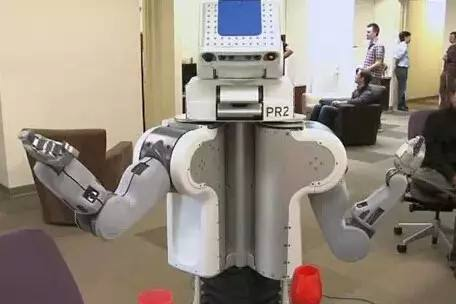
\includegraphics[height=3.5cm]{pr2.jpeg}
  \caption{PR2服务机器人}
  \label{fig:pr2}
\end{subfigure}%
\begin{subfigure}{.4\textwidth}
  \centering
  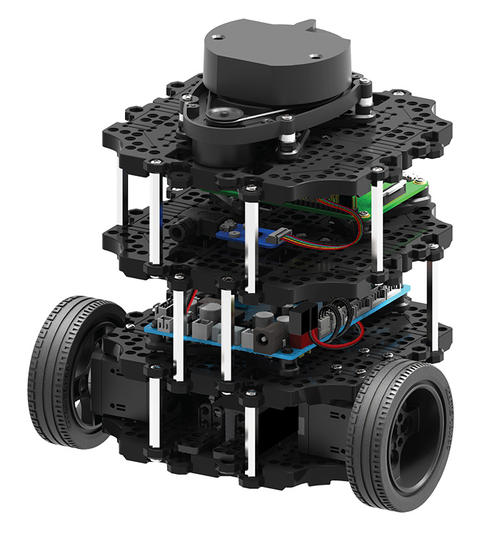
\includegraphics[height=3.5cm]{turtlebot3.jpg}
  \caption{turtlebot3机器人}
  \label{fig:turtlebot}
\end{subfigure}
\caption{学术机器人平台}
\end{figure}

为了统一机器人算法研究的编程平台,降低方法的复现难度,促进社区的健康发展。广大机器人
研究学者们也参与推动维护了多个开源的机器人编程框架,其中包括应用广泛的ROS
(Robot Operating System)\cite{quigley2009ros},YARP
(Yet another robot platform)\cite{metta2006yarp}等框架。这些开源框架为社区提供了
极大的发展便利,同时某些面向学术研究的移动机器人操作平台也通过捆绑支持这些机器人
编程框架取得了商业上的成功,例如前文提到的PR2和TurtleBot机器人;Universal Robotics
研发的URx系列机械臂\ref{fig:urx}; 以及国内的autolabor四轮
差速车\ref{fig:autolaborpro1}\ref{fig:autolabor}等等产品。


\begin{figure}
\centering
\begin{subfigure}{.6\textwidth}
  \centering
  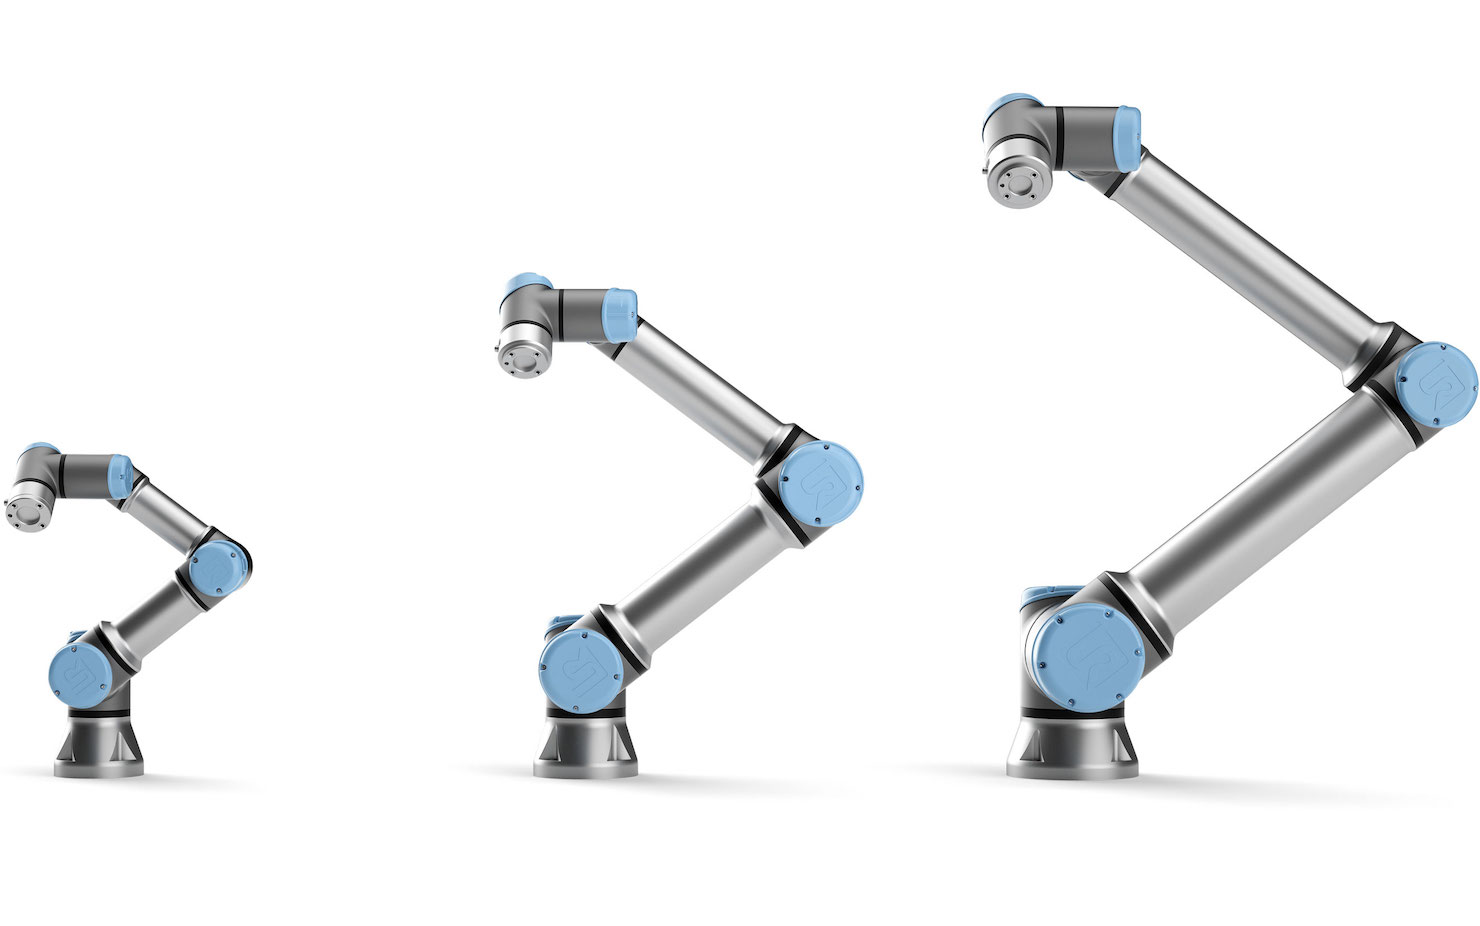
\includegraphics[height=3.5cm]{ur_series.jpg}
  \caption{Universal Robotics研发的系列UR机械臂}
  \label{fig:urx}
\end{subfigure}%
\begin{subfigure}{.4\textwidth}
  \centering
  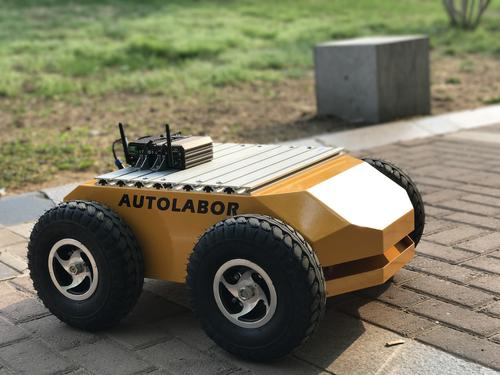
\includegraphics[height=3.5cm]{autolaborpro1.jpg}
  \caption{Autolabor 大负载四轮差速车}
  \label{fig:autolaborpro1}
\end{subfigure}
\begin{subfigure}{.5\textwidth}
  \centering
  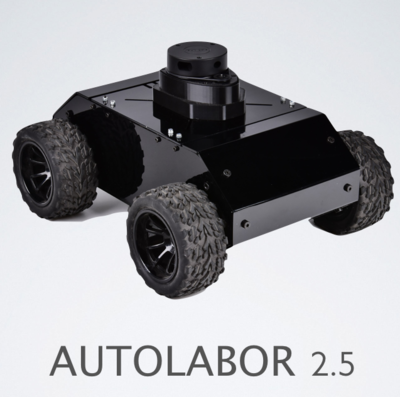
\includegraphics[width=.6\linewidth]{autolabor.jpg}
  \caption{Autolabor小型四轮差速平台}
  \label{fig:autolabor}
\end{subfigure}
\caption{支持ROS平台的机器人产品}
\end{figure}


机器人算法一直是科研领域的研究热点,按照功能可以将机器人相关的算法分为感知和控制两部分。
感知方向包括物品的检测、分类、定位等功能,得益于深度神经网络的快速发展,机器人的感知能力
近年来有了飞速的提高,借助经典的视觉检测方法配合机械臂规划方法实现的快速自动分捡方案
在各大比赛中不断出现。借助深度学习或者传统视觉方法、点云处理方法实现的拾取平面检测,抓取
点寻找,夹爪位姿寻找算法也不断涌现,并且取得了非常好的效果。在导航定位方面,SLAM技术(
simultaneous localization and mapping,即时定位与地图构建)日趋成熟,基于视觉、点云或者
多传感器融合的算法不断出现,如ORB-SLAM\cite{mur2015orb},Cartographer\cite{hess2016real},
VINS\cite{qin2018vins}等等,不断提高机器人主动定位的精度与鲁帮性。导航算法的进步主要体现
在控制框架的创新和完善上,经过数十年的努力,机器人社区在导航方面已经形成了较为稳定的一套
方法,即基于Costmap的分层地图维护方法\cite{lu2014layered}和分别负责路径生成与控制命令
生成的双规划器算法\cite{guimaraes2016ros}。目前
在静态环境中的灵活避障导航问题已经基本被解决\cite{Zhou2017A}。 此外增强学习在机器人控制
上的应用也成为近年来算法方向的研究热点\cite{schaal2002learning}。

为促进研究成果在实际场景中的应用,各大公司会议等组织举办了许多世界级的面向特定场景的
机器人大赛,其中著名的有Amazon Picking Challenge\cite{wurman2016amazon},
RoboCup@Home\cite{wisspeintner2009robocup},IROS Manipulation Competition\cite{moon2017iros}。
这些比赛极大的促进了机器人社区的交流,在比赛期间也涌现出了许多优秀的机器人设计以及
方法,例如在RoboCup@Home赛场上就出现了大量设计新奇,功能多样的机器人\ref{fig:other_teams}。

\begin{figure}
    \centering
    \begin{minipage}{.45\linewidth}
            \begin{subfigure}[t]{.9\linewidth}
                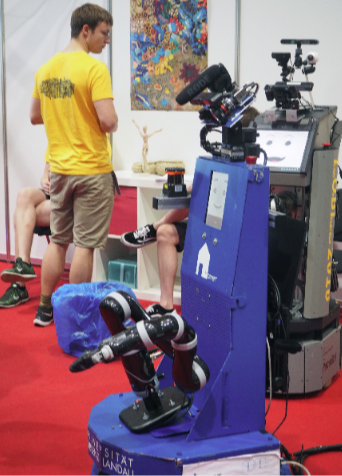
\includegraphics[width=\textwidth]{homer.png}
                \caption{homer@ UniKoblenz}
            \end{subfigure}
    \end{minipage}
    \begin{minipage}{.45\linewidth}
        \begin{subfigure}[t]{.8\linewidth}
            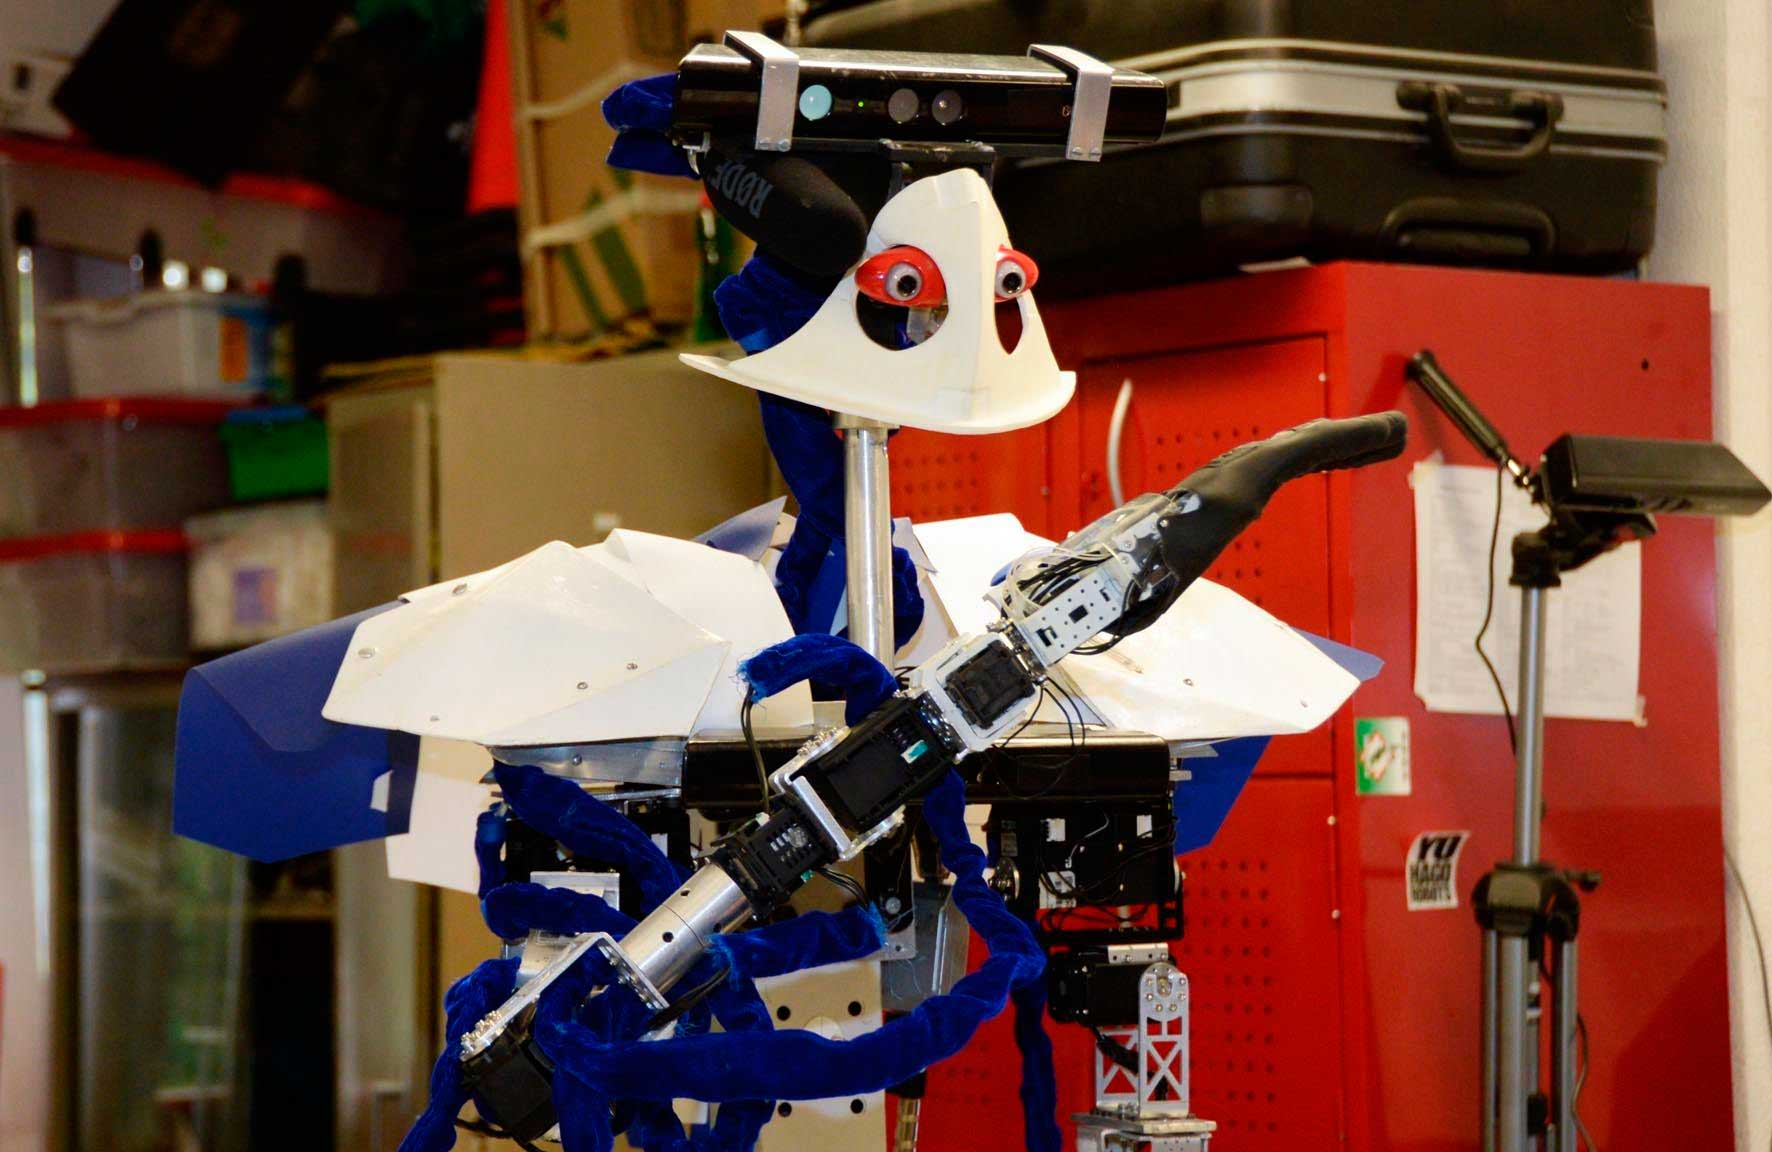
\includegraphics[width=\textwidth]{pumas.jpg}
            \caption{Pumas}
        \end{subfigure} \\
        \begin{subfigure}[b]{.8\linewidth}
            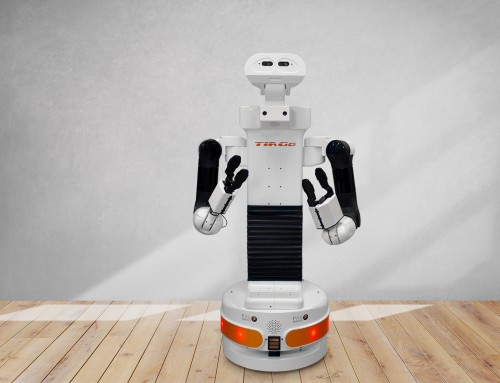
\includegraphics[width=\textwidth]{catie.jpg}
            \caption{CATIE Robotics}
        \end{subfigure} 
    \end{minipage}
    \caption{RoboCup@Home中出现的机器人}
    \label{fig:other_teams}
\end{figure}

\section{本文内容简介}

本章系统的介绍了移动操作机器人的基本定义和国内外研究、应用现状。后续章节将对本文的
主要工作——Tinker移动操作机器人进行介绍,详细的给出Tinker机器人的系统搭建,定位
导航算法的实现与调试,机械臂控制及相应的视觉算法实现以及各部分的版本迭代经过。

\iffalse
\section{Tinker机器人的设计目标}

清华大学未来机器人团队成立于2012年,旨在帮助对机器人领域各个方面感兴趣的
同学提升技术水平,增进校内交流,提供必要的设施支持,搭建一个校内的,开放有趣的机器人
交流平台。随着团队的不断发展壮大,未来机器人团队逐渐积累了相当一批技术人才,并且开始有
机会参于国际比赛。其中Tinker机器人作为团队的主要开发项目,每年固定参加著名的RoboCup
比赛@HOME分赛场\cite{wisspeintner2009robocup}。

作为清华校内机器人方向最具影响力的学生社团,未来机器人团队在促进校内机器人相关领域的
社区发展,提高同学们的技术水平方面起到了重要影响。其中Tinker作为未来机器人团队的重要
支撑项目,在凝聚团队,提升技术水平,扩大队员眼界方面起到了重要的作用。并且Tinker本身
的技术迭代和技术积累也对校内科创发展起到了极大的推动作用,这些珍贵的技术经验不仅惠及
了未来机器人团队内部成员,也广泛的影响了校内科创领域的许多组织。

\begin{figure}
  \centering
  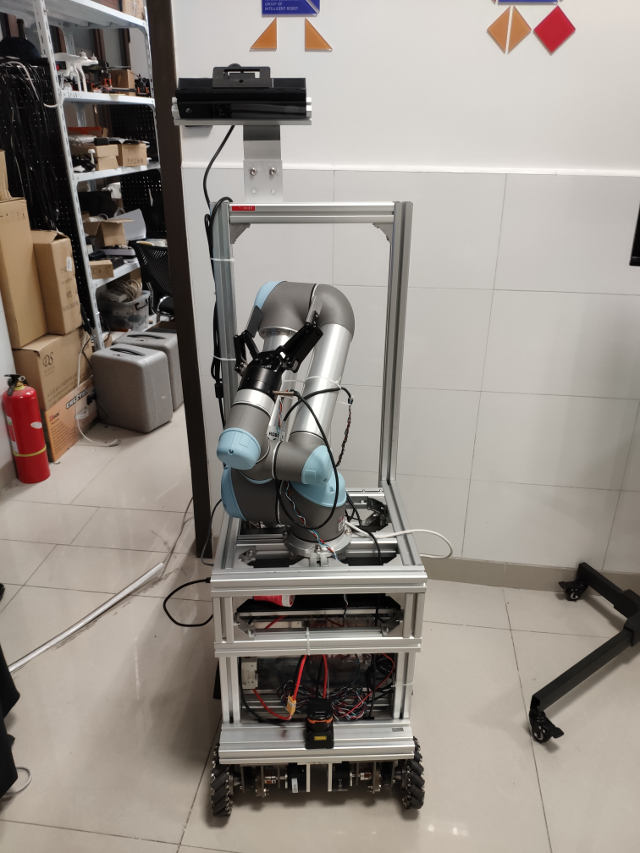
\includegraphics[width=.4\linewidth]{tinker_overview.jpg}
  \caption{Tinker外观}
  \label{fig:tinker_overview}
\end{figure}


\section{RoboCup@Home简介}

RoboCup@Home作为机器人领域的国际顶级赛事,旨在帮助提升机器人在复杂的开放环境中的表现,
促使家庭服务型机器人行业的发展。RoboCup@Home赛场分为三个联盟:Open Platform League
(OPL),Domestic Standard Platform (DSPL),Socal Standard Platform League
 (SSPL)。

三大赛事联盟中DSPL与SSPL均指定机器人的比赛,开发者不允许使用除特定机器人之外的任何机器人
参赛,且不允许替换、改装、外挂任何除机器人本身带有的部件,这两个联赛旨在促进社区内对相关
算法及软件工程的提升。其中DSPL规定使用Toyota Human Support Robot (HSR)\cite{toyota_hsr}
机器人,SSPL规定使用Softbank Robotics Pepper\cite{pandey2018mass}机器人。两款
机器人如图\ref{fig:hsr_pepper}所示。


OPL为开放平台比赛,参赛者必须自行设计搭造参赛机器人,并且为机器人编写特定的软件完成比赛
中制定的任务。OPL旨在通过开放的硬件要求培养机器人领域结构、硬件相关的人才,提升各个高校
和组织中的硬件设计能力,并探索结构、硬件方面的更多可能性。Robocup@Home自2009年开始举办,
多年的比赛中OPL赛场中涌现了大量的优秀机器人设计作品,Tinker即为其中优秀的一员。除Tinker
外,还有homer@ UniKoblenz\cite{memmesheimer2017homer},Pumas\cite{savage2013pumas},
CATIE Robotics\cite{fabre2018catie}等一批外观独特,功能强大的参赛作品出现,如图\ref{fig:other_teams}。

Robocup@Home比赛每年举行一次,举行地点在国际几大城市巡回举办,由高校或者相关组织承办。
通常比赛分为3个stage,每个stage设有若干任务,参赛队伍一次完成任务,根据完成程度和完成时
的表现(速度,流畅性等等)按点得分,分数靠前的队伍可以获得晋级资格,进入下一stage。stage I
为基础功能比赛,主要考察避障导航、抓取、识别、语音交互等基础功能,辅以合理的机器人软件控制
程序即可完成,这一个stage主要考察机器人基本的软硬件设计的自恰性及稳定性,相当多新手队伍会
在stage I直接淘汰。

stage II的任务内容同stage I基本相当,但是难度会更高,逻辑也更复杂,特别的,在近几年的比赛中,
增加了General Purpose Service Robot(GPSR)任务,即裁判对机器人下达任意在Robocup@Home
赛场上曾经出现过的任务,考察机器人的完成情况,这一任务旨在帮助参赛者更好的构建机器人控制
软件,为家用机器人在真实场景下的应用做铺垫。

Final stage为两个得分最高的团队关于冠军奖项的争夺,每年的任务并不固定,2020年组委会
将送餐机器人作为Final Stage的考察目标,要求参赛队伍在一个嘈杂的餐厅环境中将食物托盘
送到某一个特定食客手上,并完成必要的交互。


\section{RoboCup@Home比赛规则介绍}

经过多年的发展RoboCup@Home已经培育起一个完善的社区,每年RoboCup@Home的比赛任务
即由社区相关人员协助商议决定,RoboCup@Home组委会共同维护一份RuleBook\cite{rulebook}
,组委会成员
使用GitHub完成RuleBook的编写任务,该仓库是完全开放且欢迎参赛者提交修改与贡献的。
RoboCup@Home组委会中,设有专门的任务制定部门Technical Committee(TC),这部分成员
大都有深厚的相关从业背景和多年的研究经验,另外有一部分成员来自各个主力参赛队伍的
核心开发人员(比如笔者作为Tinker机器人的主要程序员参与了2020年的TC工作),以
确保比赛规则同时兼顾学科研究热点和可完成性。

随着机器人行业相关技术的不断发展,RuleBook中的任务也在每年更新,并且向着越来越复杂、
越来越贴近真实生活场景的方向演进。在多年的比赛中,组委会在任务内容、任务形式上也作出
了很多改进与尝试,2019年的RoboCup@Home比赛就及其大胆的将任务数量进行了爆炸式的扩容,
尝试了很多新的复杂的任务,其中有一些被证明并不成功,因此2020年的规则制作过程中又将
不合理的任务去除,将任务数量固定为Stage I 5个,Stage II 4个。

\subsection{RoboCup@Home经典任务分析}




\section{Tinker的历史版本}

在近5年的参赛过程中,Tinker机器人经过机器人队几代同学的不断开发,经历了若干次迭代,
其硬件设计、软件架构、传感器使用、方案选择都发生了本质的变化。在Tinker不断迭代的
过程中,机器人队也积累了大量的相关经验和教训,培养出了一代代机器人相关的人才。

早期机器人团队技术实力差资金紧张,因此我们自制了整个机器人参加比赛。当时的机器人如图
\ref{fig:old_tinker}所示。当时的虽然工艺粗糙,精度很低,但是辅以合适的
软件算法和恰当的策略,仍然在RoboCup的赛场上取得了不错的成绩。当时的队员们如今有的
已经走上工作岗位,有的还留在学校继续攻读更高的学位,都在各自的领域中继续发挥自己的
能量。


\begin{figure}[H]
\centering
\begin{subfigure}{.5\textwidth}
  \centering
  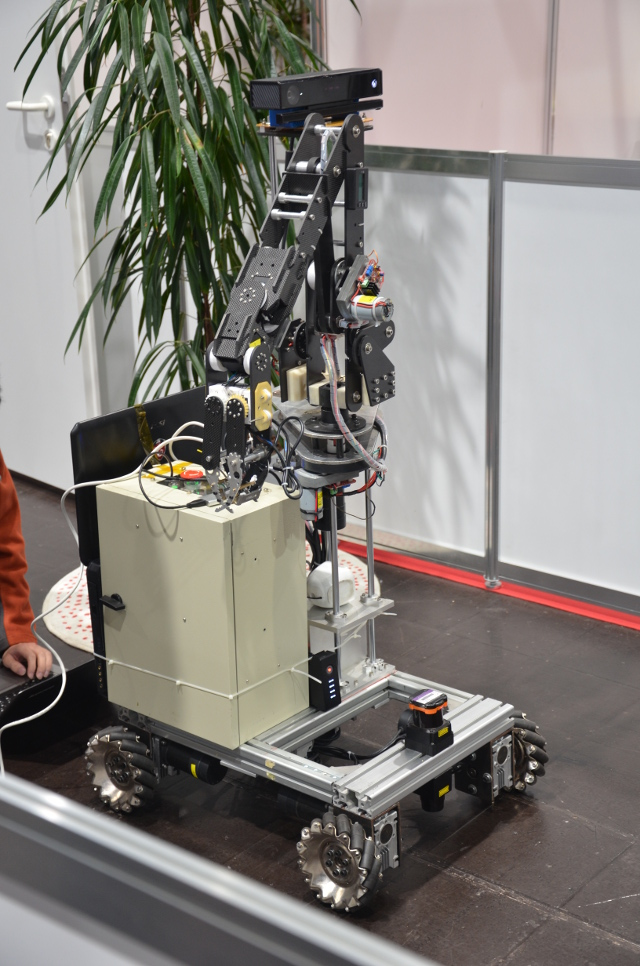
\includegraphics[width=.6\linewidth]{old_tinker1.jpg}
  \caption{早期Tinker侧视图}
\end{subfigure}%
\begin{subfigure}{.5\textwidth}
  \centering
  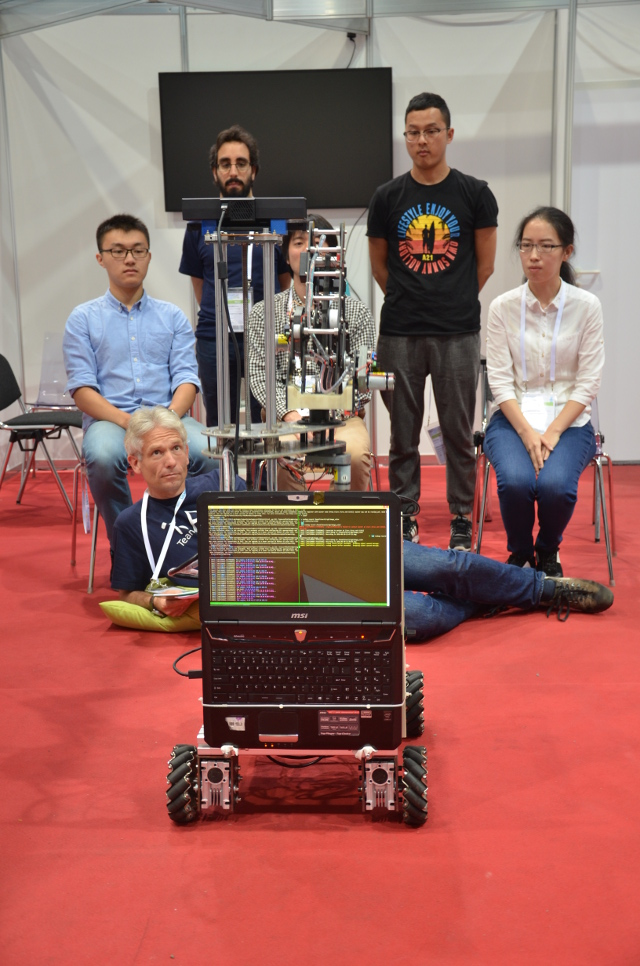
\includegraphics[width=.6\linewidth]{old_tinker2.jpg}
  \caption{早期Tinker主视图}
\end{subfigure}
\begin{subfigure}{.8\textwidth}
  \centering
  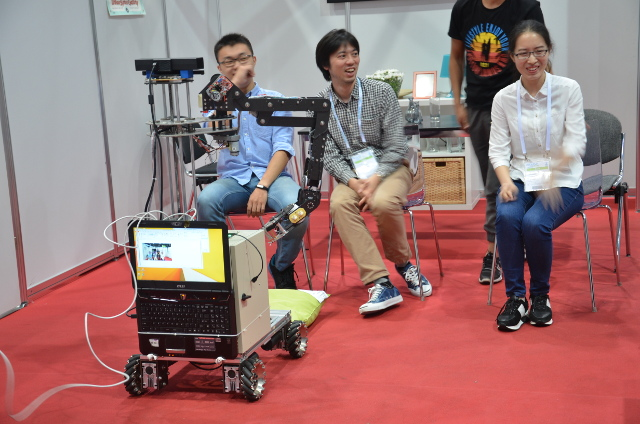
\includegraphics[width=.7\linewidth]{old_tinker3.jpg}
  \caption{早期Tinker在赛场上}
\end{subfigure}
\caption{RoboCup@Home指定机器人,左HSR 右Pepper}
\label{fig:old_tinker}
\end{figure}

经过几年的积累,机器人团队于2019年对Tinker进行了彻底的改装,包括
使用市售成品机械臂及夹爪、使用更高性能的笔记本个更高性能的电机等等
改造,外观如图\ref{fig:tinker1}。硬件的大幅改进对机器人开发带来
了极大的冲击,新版Tinker最初
的很多设计并不合适,因此经过2019年RoboCup@Home比赛后,我们又对Tinker
进行了一次大规模的改装。第二次改装吸取了前面的教训,大幅裁剪了很多
冗余设计,改良了供电和控制电路方案。在软件上也有诸多变化,一方面
固化了许多经过前人验证的优良开发范式,一方面积极缩减代码依赖,在
轻量化和稳定性方面不断提高,以争取更好的赛场表现。改装后的Tinker外观
如图\ref{fig:tinker2}所示。

\begin{figure}
\centering
\begin{subfigure}{.5\textwidth}
  \centering
  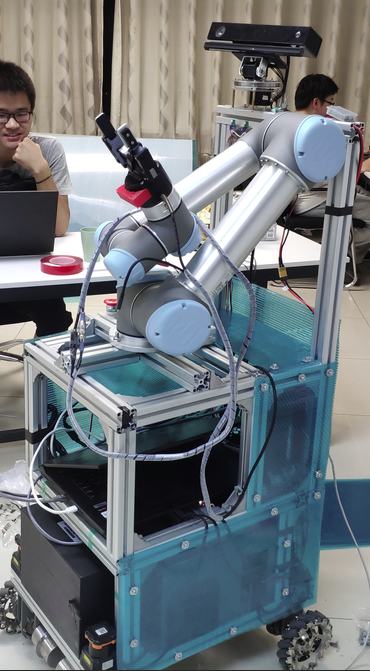
\includegraphics[width=.6\linewidth]{tinker1.png}
  \caption{改装Tinker 1.0}
  \label{fig:tinker1}
\end{subfigure}%
\begin{subfigure}{.5\textwidth}
  \centering
  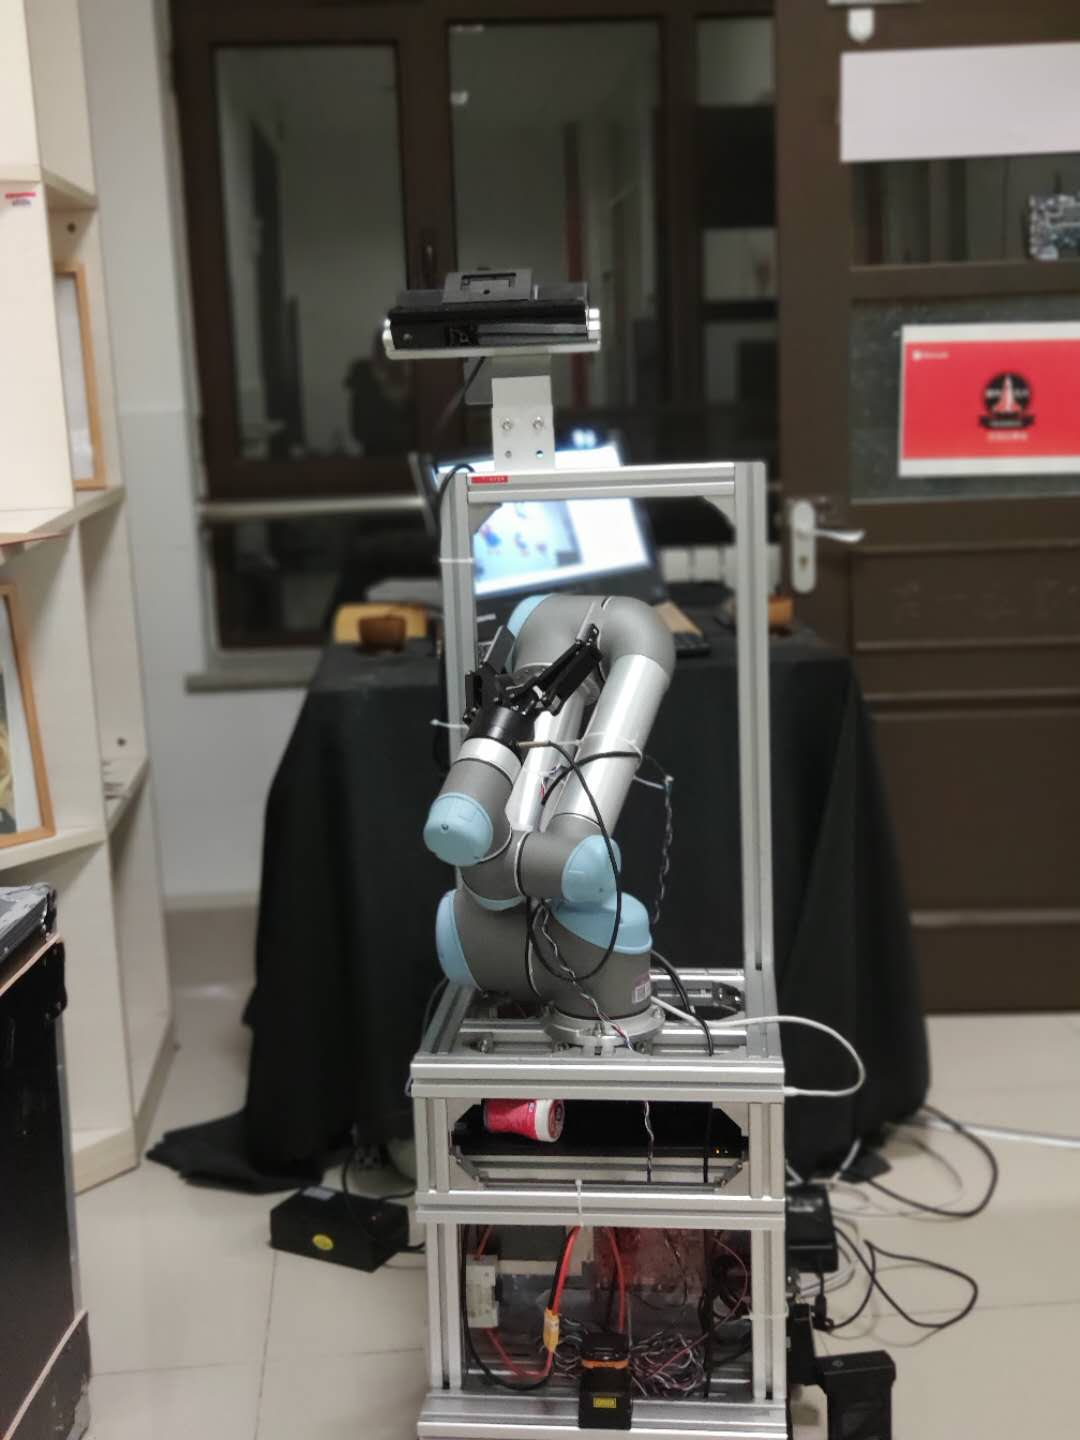
\includegraphics[width=.6\linewidth]{tinker2.jpg}
  \caption{改装Tinker 2.0}
  \label{fig:tinker2}
\end{subfigure}
\caption{新版Tinker二次改装前后的外观,左改装前,右改装后}
\label{fig:tinker_new}
\end{figure}




\fi









